\documentclass[]{article}
\usepackage{amsmath}
\usepackage{listings}
\usepackage{float}
\usepackage[framed,numbered,autolinebreaks,useliterate]{mcode} 
\usepackage[dvipdfm]{graphics}
\usepackage[dvipdfm]{graphicx}
\usepackage{color}
\DeclareGraphicsExtensions {.eps ,.mps ,.pdf ,.jpg ,.png}

%opening
\title{Computer Project}
\author{Student}
\date{\today}

\begin{document}

\maketitle

\section{a.Gradient Method}
\subsection{Analytical expression for the gradient}
For $$f(\mathbf{x}) = -\sum_{i=1}^m\ln(1-\mathbf{a}_i^T\mathbf{x})-\sum_{i=1}^n\ln(1-x_i\phantom{}^2)$$ the gradient of $f(\mathbf{x})$ is $\nabla f(\textbf{x})=\frac{\partial f(\mathbf{x})}{\partial x_i}\mathbf{e}_i$ 
\par For the $k$-th component of the gradient vector , $$\frac{\partial f(\mathbf{x})}{\partial x_k}\mathbf{e}_k = \left(\sum_{i=1}^m\frac{(\textbf{a}_i)_k}{(1-\textbf{a}_i^T\textbf{x})} + \frac{2x_k}{(1-x_k\phantom{}^2)}\right) \textbf{e}_k$$ where $(\textbf{a}_i)_k$ denotes the $k$-th component of the vector $\textbf{a}_i$, which is a scaler. 
\par Tightly expressed, we have:
$$\nabla f(\textbf{x}) = \sum_{i=1}^m\frac{\textbf{a}_i}{(1-\textbf{a}_i^T\textbf{x})}+2(\textbf{I}-\mathrm{diag}(x_k\phantom{}^2))^{-1}\textbf{x}$$ where $k $ is the component parameter of the diagonal matrix, shown as: $$\mathrm{diag} (x_k\phantom{}^2) = \left(\begin{matrix}
x_1\phantom{}^2&&&\\
&x_2\phantom{}^2&&\\
&&\ddots&\\
&&&x_n\phantom{}^2
\end{matrix}\right) $$
\subsection{Solve the problem}
For the Gradient Descent Method with backtracking line search, where $0<\alpha<0.5$ and $0<\beta<1$: 
\par The iterative equations are :
$$\left\{\begin{array}{l}
\textbf{x}^0 = \textbf{0}\\
\Delta \textbf{x} = -\nabla f(\textbf{x})\big|_{\mathbf{x}^i}  \\
t_i = \text{find\_backtracking\_step}(\textbf{x}^i)\\
\textbf{x}^{i+1} = \textbf{x}^i + t_i\Delta \textbf{x}\\
\end{array}\right.$$
\par The terminated condition is :
$$||\nabla f(\textbf{x})||_2\le \eta \quad \text{at iterative step} \; i$$
\par The result then is 
$$f(\textbf{x}) = f(\textbf{x}^i)$$
\par The methond of finding backtracking step given $\textbf{x}^i$ are:

$$\left\{\begin{array}{l}
t_0 = 1\\
t_{k+1} = \beta t_k \quad \mathrm{iff.}\; f(\mathbf{x}^i + t_k \Delta\mathbf{x}) > f(\mathbf{x^i})+\alpha t_k\nabla f(\mathbf{x})^T\Delta\textbf{x}
\end{array}\right.$$

The terminated condition is :
$$f(\textbf{x}+ t_k\Delta\textbf{x}) \le f(\textbf{x})+\alpha t_k\nabla f(\textbf{x})^T\Delta\textbf{x}\quad \text{at step} \; k$$
\par And the return value of find\_backtracking\_step$(\textbf{x}_i)$ is $t_k$.
\subsubsection{code}


\begin{lstlisting}	
%Gradient Method

% initialize 
clear all;
alpha = 0.1;
beta = 0.6;
eta = 1e-5;


% generate the random instance

global A;
%load('A_200_100.mat');
load('A_500_400.mat')
[m ,n] = size(A);

value = [];
step = [];
%main iteration


% at step 0
x = zeros(n,1);
grad = A'*(1./(1 - A*x)) - 1./(1+x) + 1./(1-x);


while norm(grad,2) > eta

value = [value, func(x)];
delta_x = -grad;
t = 1;

% constrain the x in dom(x) by changing t
while ((max(A*(x+t*delta_x)) >= 1) || (max(abs(x+t*delta_x)) >= 1))
t = t * beta;
end

% backtracking line search 
while (func(x+t*delta_x) - func(x) > alpha * t * grad' * delta_x)
t = t * beta;
end
step = [step, t];
% update x by:
x = x + t * delta_x; 
% update new gradient at x by:
grad = A'*(1./(1 - A*x)) - 1./(1+x) + 1./(1-x);
end 

%dump result
opt = min(value);

figure(1)
subplot(1,3,1);
plot([0:(length(value)-2)], value(1:length(value)-1), '-');
yl = '$f(\textbf{x}^k)$';
xlabel('iterative step');
ylim([min(value) max(value)]);
ylabel(yl,'Interpreter','latex');
title('value - iterative step');

hold on;

subplot(1,3,2);
semilogy([0:(length(value)-2)], value(1:length(value)-1)-opt, '-');
xlabel('iterative step');
yl2 = '$f(\textbf{x}^k)-p^*$';
ylabel(yl2,'Interpreter','latex');
title('value between opt - iterative step');

hold on;

subplot(1,3,3);
scatter([1:length(step)], step,'filled','black');
xlabel('iterative step'); 
ylabel('$t^k$','Interpreter','latex');
title('step size - iterative step')
hold on;

function res = func(x)
global A;
res = -sum(log(1-A*x)) - sum(log(1+x)) - sum(log(1-x));
end

%
%

\end{lstlisting}

\subsection{Result}
In this case and the following experimemt, we use totally two normal instance (not testing the parameter of BLS or the convergency). The small instance is with $m=200, n=100$ and the large instance is with $m=500,n=400$, the vector set of $\mathbf{a}_i$ are equipped as matrix, and each element are generated as random number.
\par Both case have the BLS parametera at $\alpha = 0.1, \beta = 0.6$.
\par The following result shows the normal testing case with three subfigure. These are function value , value towards optimal value and time step size to iterative step number. The second figure value towards optimal value to iterative step number are plot in $y$  - logarithmic axis. \color{blue} Because the function value have negative true value, we can not plot the first figure in $y$  - logarithmic axis.
\color {black}

\begin{figure}[H]
	\centering
	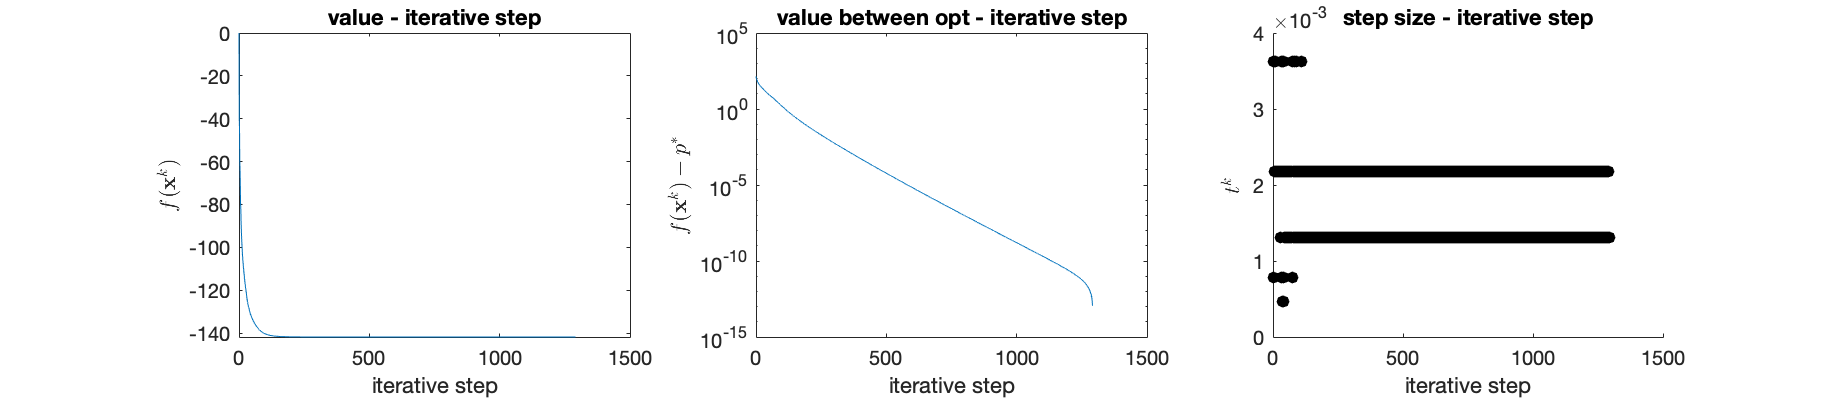
\includegraphics[width=350pt,keepaspectratio]{Gra_small_normal}
	\caption{Instance 1, small instance}
\end{figure}

\begin{figure}[H]
	\centering
	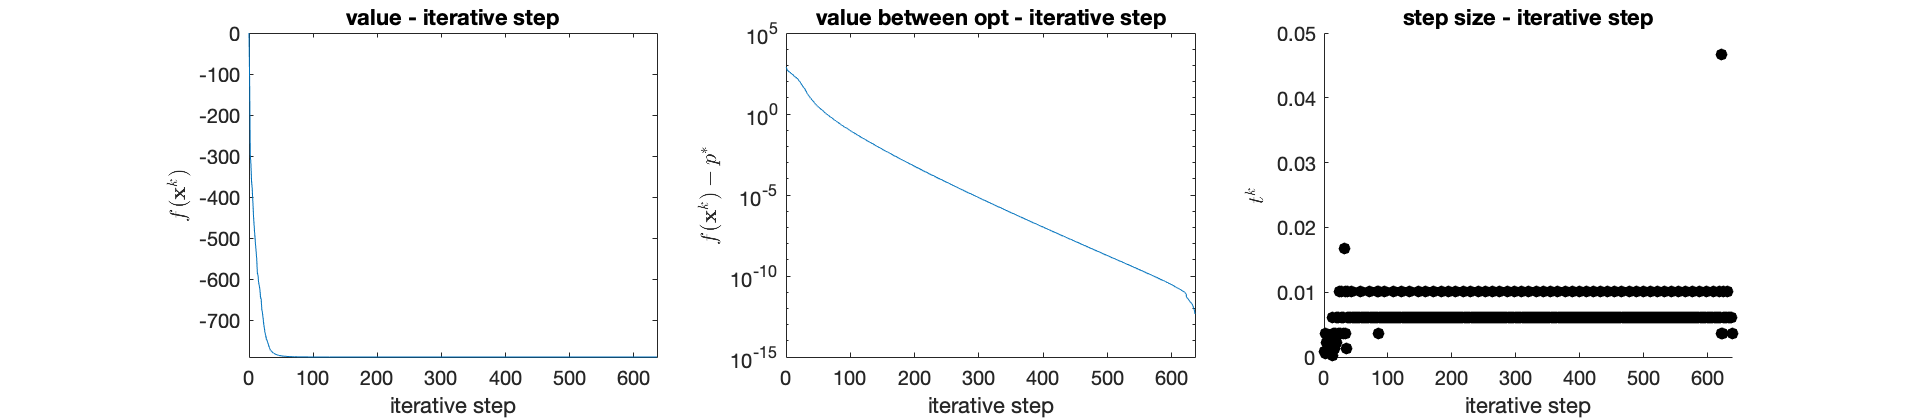
\includegraphics[width=350pt,keepaspectratio]{Gra_large_norm}
	\caption{Instance 2, large instance}
\end{figure}
\subsubsection{BLS parameter}
The backtracking line search have two parameter $\alpha, \beta$. The BLS is a algorithm finding the maximize $t$ with a constraint which ensure the next step closer enough towards the optimal without marching to large step in a specific step direction.
\par The following results show the parameter impact.
\par We use blue line as base line, with \color{red} \textbf{$\alpha = 0.45, \beta = 0.85$}.\color{black}
\begin{figure}[H]
	\centering
	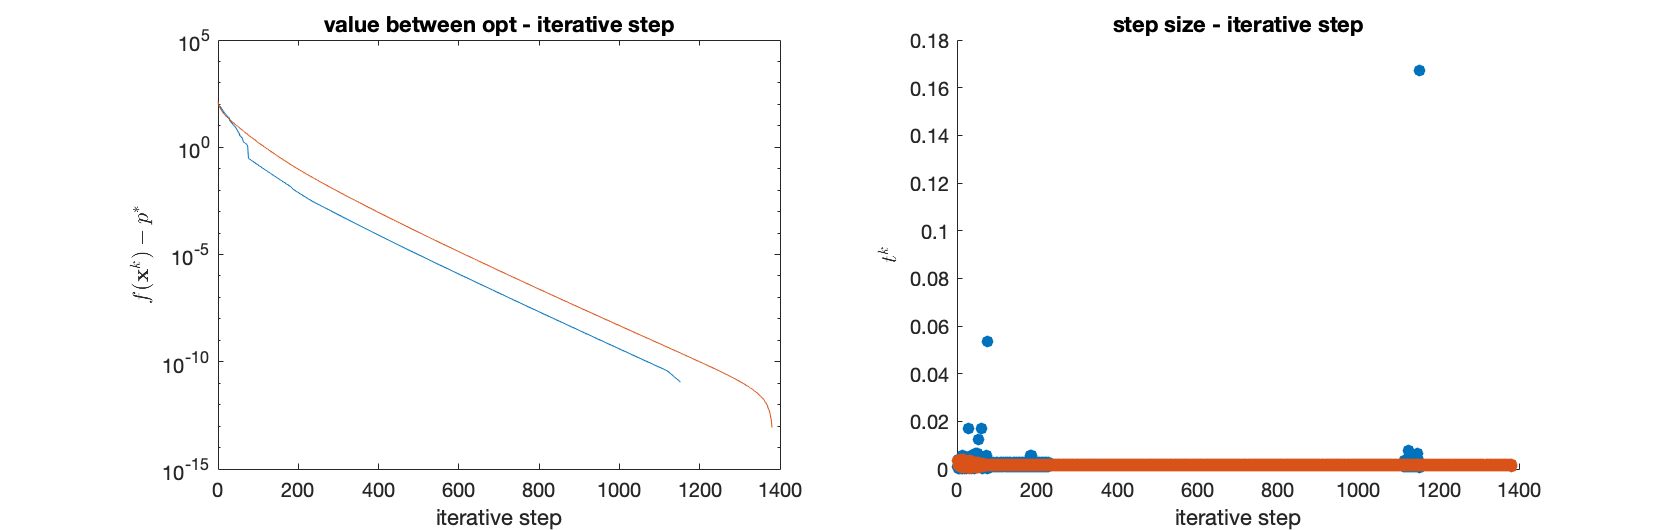
\includegraphics[width=350pt,keepaspectratio]{ga1_45_b85}
	\caption{tryout 1, various  $\alpha$}
\end{figure}
For the orange case, the $\alpha = 0.1$. The smaller $\alpha$ makes the step along a step direction closer to the  coutor line, and this leads small step size. So the iterative step will grow.

\begin{figure}[H]
	\centering
	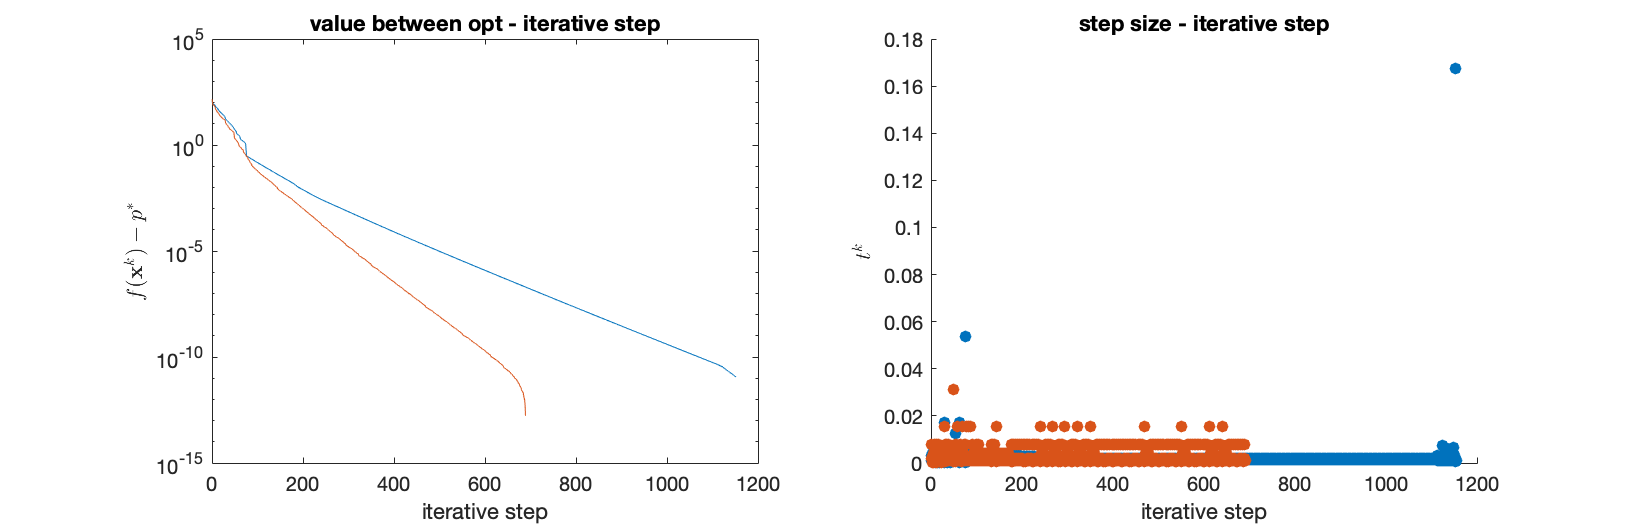
\includegraphics[width=350pt,keepaspectratio]{ga45_b5_85}
	\caption{tryout 2, various $\beta$}
\end{figure}
For the orange case, the $\beta = 0.5$. The smaller $\beta$ have faster run time, because it iterates the $t$  with large damping. And because the $t $ damped fast, which means a great progress, the stop condition of BLS maybe reach with rough accuracy, which makes step size fall into a larger value(because when reach the condition, the t will not update and stay in the last $t$) than its exact value. So the total iterative step become smaller for a specific error.

\section{b.Damped Newton's Method}
\subsection{Analytical expression for the Hessian}
The Hessian of this problem is $$\textbf{H}:=\nabla^2 f(\textbf{x}) = \sum_{i=1}^{m}\frac{\textbf{a}_i\textbf{a}_i^T}{(1-\textbf{a}_i^T\textbf{x})}+\mathrm{diag}\left(\frac{2(1+x_k\phantom{}^2)}{(1-x_k\phantom{}^2)^2}\right)$$ note that $\textbf{a}_i\textbf{a}_i^T$ is outer product and returns a matrix.
\subsection{Solve the problem}
The only difference towards case \textbf{1 a} is that $\Delta \textbf{x}$ is given as 
$$\Delta \textbf{x}_{\mathrm{dnt}} =  -\textbf{H}^{-1}\nabla f(\textbf{x})$$
\par And the stopping criterion is $\frac{1}{2}\lambda{(\mathbf{x})}^2\le \epsilon$, where
$$\lambda{(\mathbf{x})}^2 := \nabla f(\textbf{x})^T\nabla^2 f(\textbf{x})^{-1}\nabla f(\textbf{x})$$
\subsubsection{code}
\begin{lstlisting}	
% damped Newton Method

clear all;
alpha = 0.1;
beta = 0.6;
epsilon = 1e-8;


% generate the random instance
global A;
%load('A_200_100.mat');
load('A_500_400.mat');
[m ,n] = size(A);
value = [];
step = [];
%main iteration


% at step 0
x = zeros(n,1);
grad = A'*(1./(1 - A*x)) - 1./(1+x) + 1./(1-x);

hessian = A'*diag((1./(1-A*x)).^2)*A + diag(1./(1+x).^2 + 1./(1-x).^2);

while 0.5 * lambda(hessian, grad) > epsilon

value = [value, func(x)];
delta_x = -hessian^(-1) * grad;
t = 1;

% constrain the x in dom(x) by changing t
while ((max(A*(x+t*delta_x)) >= 1) || (max(abs(x+t*delta_x)) >= 1))
t = t * beta;
end

% backtracking line search 
while (func(x+t*delta_x) - func(x) > alpha * t * grad' * delta_x)
t = t * beta;
end
step = [step, t];
% update x by:
x = x + t * delta_x; 
% update new gradient and hessian at x by:
grad = A'*(1./(1 - A*x)) - 1./(1+x) + 1./(1-x);
hessian = A'*diag((1./(1-A*x)).^2)*A + diag(1./(1+x).^2 + 1./(1-x).^2);

end 

%dump result
opt = min(value);

figure(1)
subplot(1,3,1);
plot([0:(length(value)-2)], value(1:length(value)-1), '-');
yl = '$f(\textbf{x}^k)$';
xlabel('iterative step');
ylim([min(value) max(value)]);
ylabel(yl,'Interpreter','latex');
title('value  - iterative step');
hold on;

subplot(1,3,2);
semilogy([0:(length(value)-2)], value(1:length(value)-1)-opt, '-');
xlabel('iterative step');
yl2 = '$f(\textbf{x}^k)-p^*$';
ylabel(yl2,'Interpreter','latex');
title('value between opt - iterative step');
hold on;

subplot(1,3,3);
scatter([1:length(step)], step,'filled','black');
xlabel('iterative step'); 
ylabel('$t^k$','Interpreter','latex');
title('step size - iterative step');
hold on;



function res = func(x)
global A;
res = -sum(log(1-A*x)) - sum(log(1+x)) - sum(log(1-x));
end

function res = lambda(hess, grad)
res = grad' * hess^(-1) * grad;
end

%
%

\end{lstlisting}
\subsection{Result}
The following figure show the result of same two instances in \textbf{case 1a}, with $\eta = 1e-8$.There are only fews iterative step remains to reach convergency.
\begin{figure}[H]
	\centering
	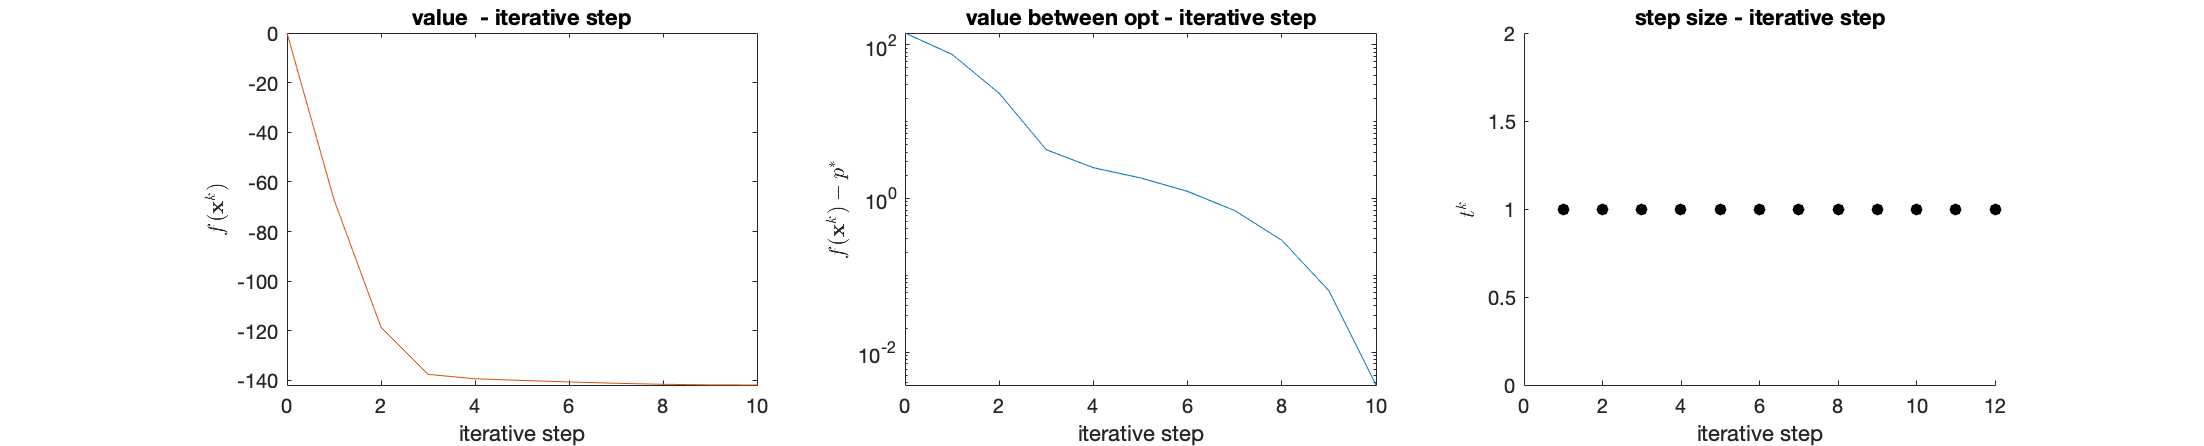
\includegraphics[width=350pt,keepaspectratio]{dnt_small_normal}
	\caption{Instance 1, small instance}
\end{figure}

\begin{figure}[H]
	\centering
	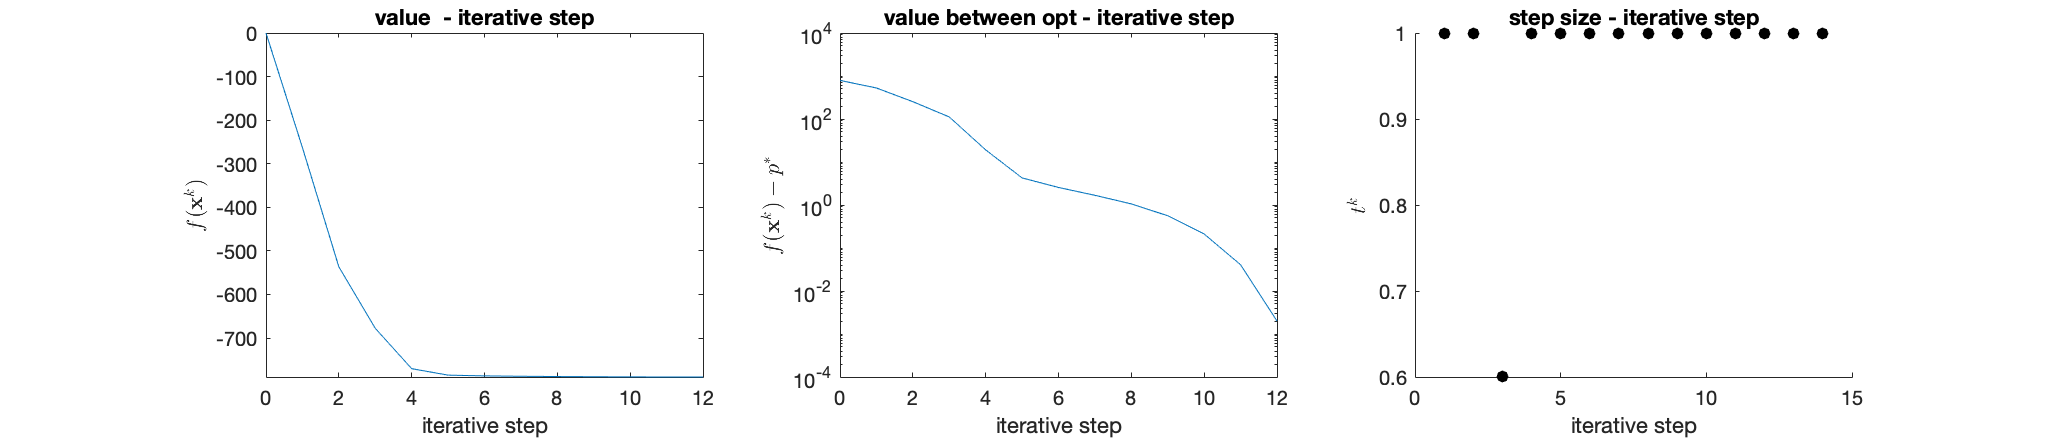
\includegraphics[width=350pt,keepaspectratio]{dnt_large_normal}
	\caption{Instance 2, large instance}
\end{figure}
\subsubsection{Convergency}
The choose of $\eta$ will depend convergency and iterative step.
\begin{figure}[H]
	\centering
	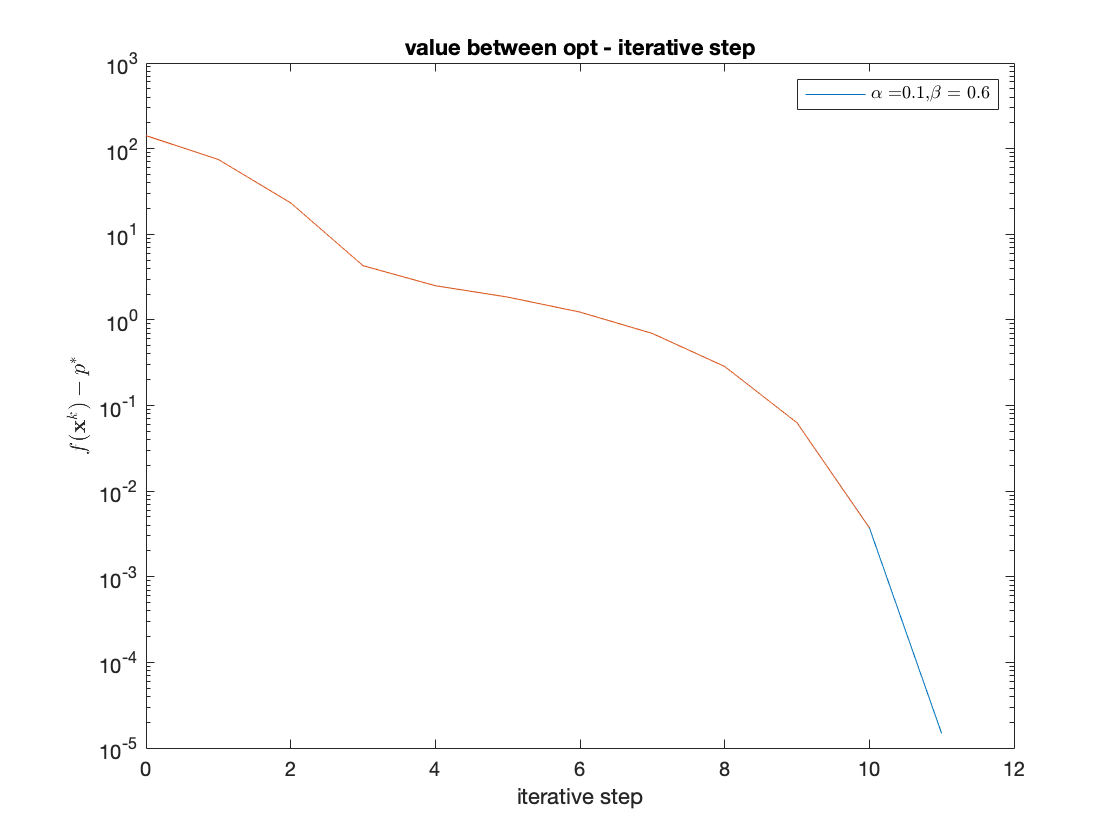
\includegraphics[width=225pt,keepaspectratio]{N}
	\caption{Different $\eta$}
\end{figure}
\par We choose $\eta = 1e-5 $ and $\eta=1e-15$, the result shows that  few extra step are needed to reach higher  error magnitude, because damped Newton Method have quadratic convergency.
\section{c.Approximated Newton's Method}
\subsection{Re-using the Hessian}
In this case, the iterative equations and terminated condition are the same as case \textbf{2 b}. The only difference is that the Hessian are updated every $N$ step, with $\Delta \textbf{x} = -\textbf{H}^{-1}\nabla f(\textbf{x})$, where $\textbf{H}$ is the last Hessian evaluted.
\subsection{code}
\begin{lstlisting}
%approximated damped Newton Method by reduce hessian calc
clear all;
% initialize 
alpha = 0.1;
beta = 0.6;
epsilon = 1e-8;


% generate the random instance
global A;
%load('A_200_100.mat');
load('A_500_400.mat');
[m,n] = size(A);
value = {};
step = {};
%main iteration

index = 1;
%do three time
for N = [1,10,40]
% at step 0

value{index} = [];
step{index} = [];
inner_step = 0;
x = zeros(n,1);
grad = A'*(1./(1 - A*x)) - 1./(1+x) + 1./(1-x);
hessian = A'*diag((1./(1-A*x)).^2)*A + diag(1./(1+x).^2 + 1./(1-x).^2);
hessian_i = hessian ^(-1);
while 0.5*lambda(hessian_i, grad) > epsilon


value{index} = [value{index}, func(x)];
delta_x = -hessian_i * grad;
t = 1;

% constrain the x in dom(x) by changing t
while ((max(A*(x+t*delta_x)) >= 1) || (max(abs(x+t*delta_x)) >= 1))
t = t * beta;
end

% backtracking line search 
while (func(x+t*delta_x) - func(x) > alpha * t * grad' * delta_x)
t = t * beta;
end
step{index} = [step{index}, t];
% update x by:
x = x + t * delta_x; 
% update new gradient at x by:
grad = A'*(1./(1 - A*x)) - 1./(1+x) + 1./(1-x);

% update new hessian and inverse at x by every N step:
if (mod(inner_step ,N) == 0)
hessian = A'*diag((1./(1-A*x)).^2)*A + diag(1./(1+x).^2 + 1./(1-x).^2);
hessian_i = hessian ^ (-1);
end
inner_step = inner_step + 1;
end 
index = index + 1;

end

%dump result
opt = min(value{3});


figure(1)
N = [1,10,40];
for i = 1:3
subplot(3,3,i);
plot([0:(length(value{i})-2)], value{i}(1:length(value{i})-1), '-');
yl = '$f(\textbf{x}^k)$';
xlabel('iterative step');
ylim([min(value{i}) max(value{i})]);
ylabel(yl,'Interpreter','latex');
title(['N=' num2str(N(i))]);
hold on;
end

for i = 1:3
subplot(3,3,i+3)
semilogy([0:(length(value{i})-2)], value{i}(1:length(value{i})-1)-opt, '-');
xlabel('iterative step');
yl2 = '$f(\textbf{x}^k)-p^*$';
ylabel(yl2,'Interpreter','latex');
title(['N=' num2str(N(i))]);
hold on;
end

for i = 1:3
subplot(3,3,i+6)
scatter([1:length(step{i})], step{i},'filled','black');
xlabel('iterative step'); 
ylabel('$t^k$','Interpreter','latex');
title(['N=' num2str(N(i))]);
hold on;
end

function res = func(x)
global A;
res = -sum(log(1-A*x)) - sum(log(1+x)) - sum(log(1-x));
end

function res = lambda(hess_i, grad)
res = grad' * hess_i * grad;
end

%
%
\end{lstlisting}
\subsubsection{Result}
This figures shows the result using different N as interval to update the hessian and its inverse.The are taken $1,10,40$. Both small and large instance are used. When $N=1$, this case is the same as \textbf{case 2b} , the damped Newton method.
\begin{figure}[H]
	\centering
	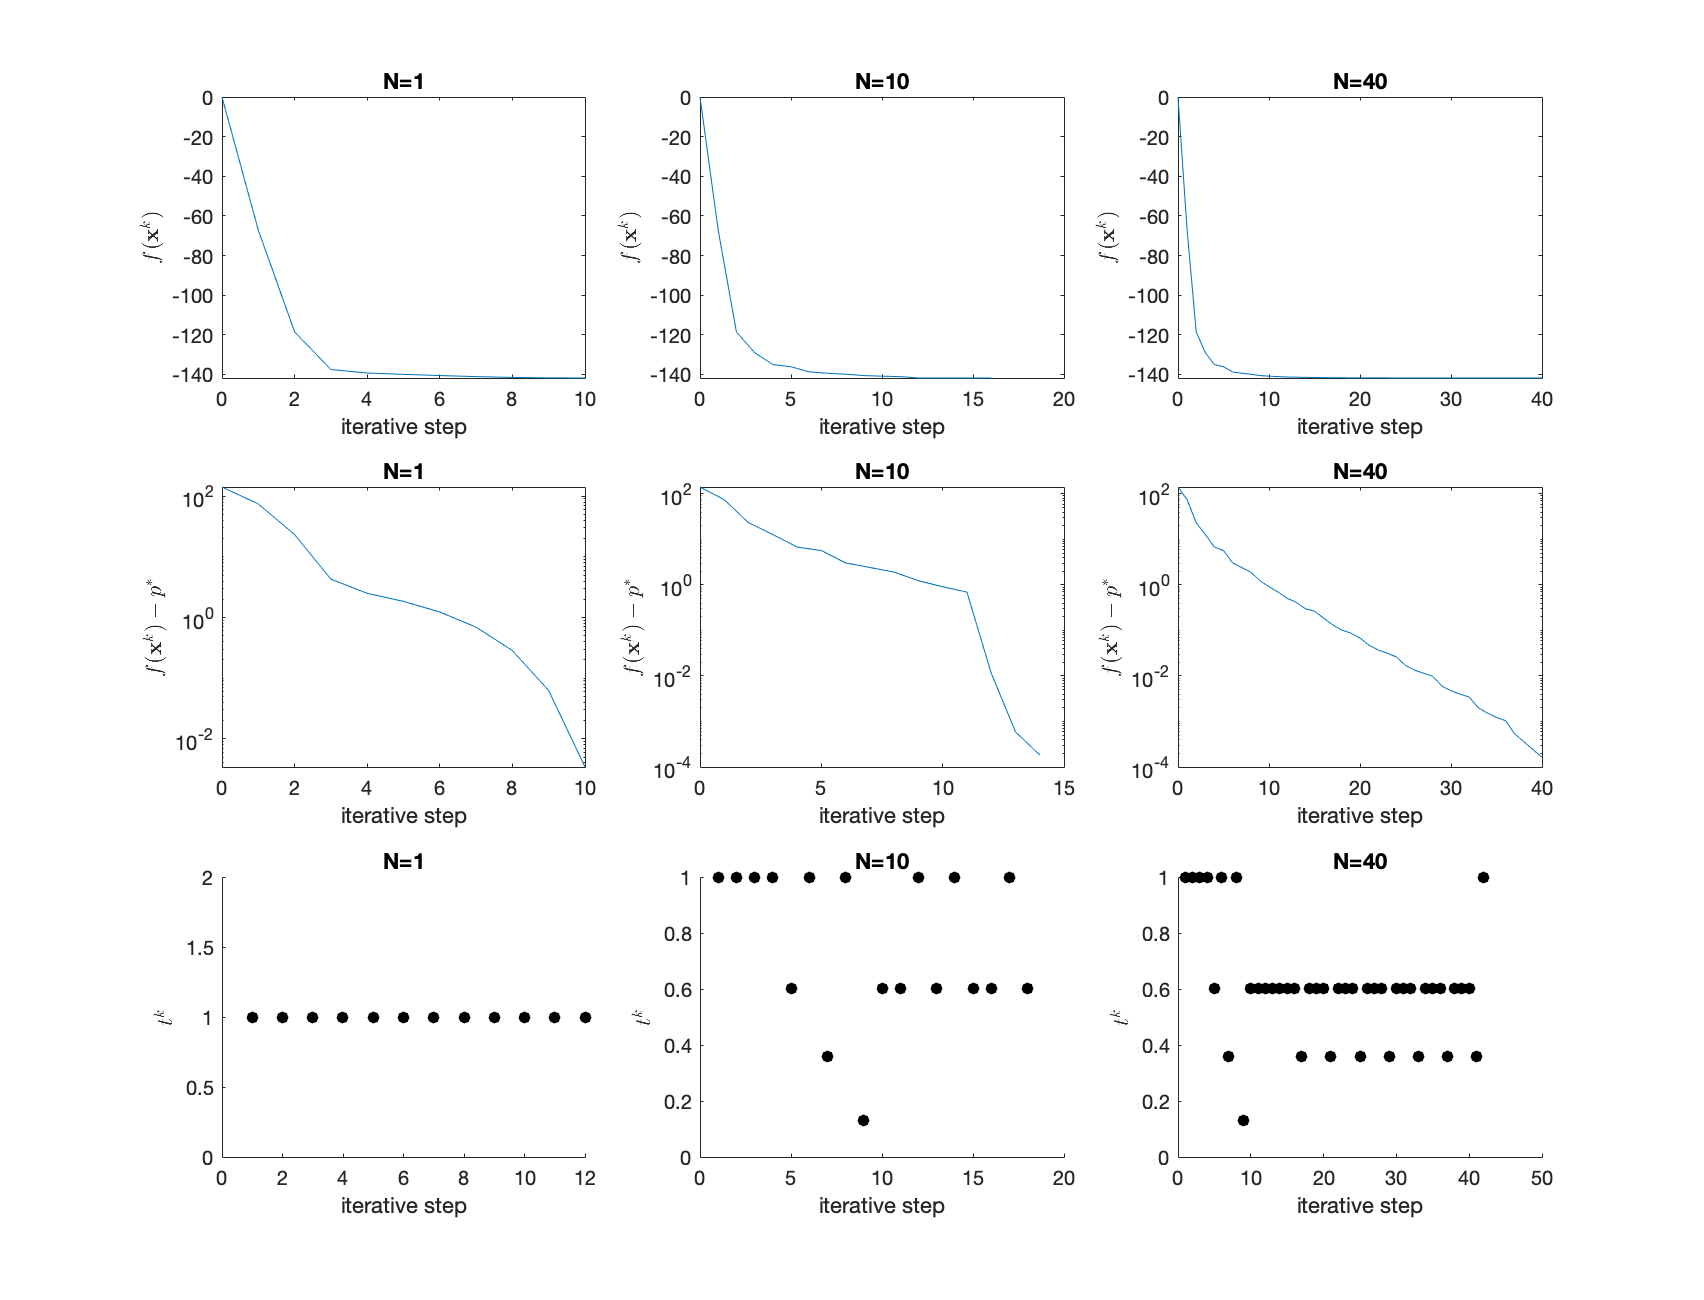
\includegraphics[width=350pt,keepaspectratio]{dampN1_small}
	\caption{Instance 1, small instance}
\end{figure}

\begin{figure}[H]
	\centering
	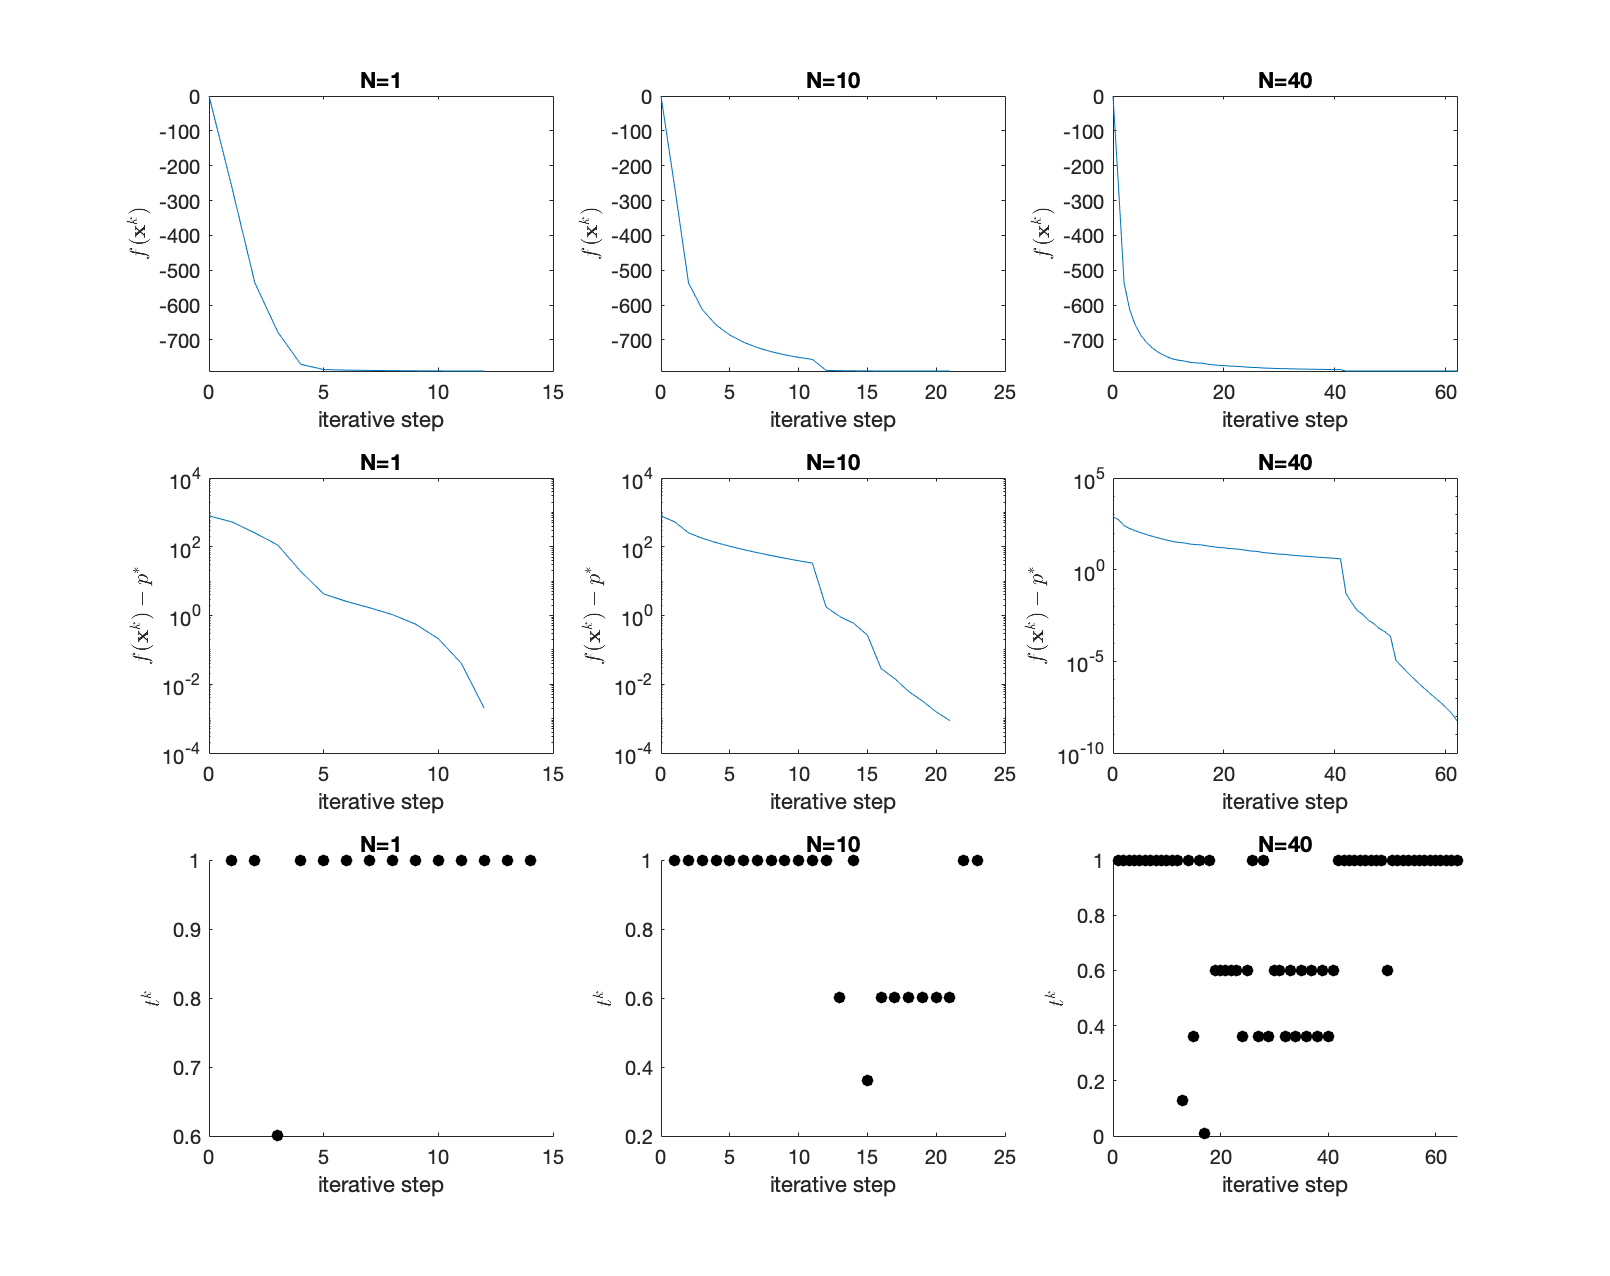
\includegraphics[width=350pt,keepaspectratio]{dampN1_large}
	\caption{Instance 2, large instance}
\end{figure}
\par From the result can we know that, the large interval remains long iterative step for a specific error limit.

\subsection{Diagonal approximation}
In this case, the iterative equations and terminated condition are the same as case \textbf{2 b}. The only difference is that the Hessian \textbf{H} is approximated as its diagonal. That is :
$$\tilde{\textbf{H}} = \mathrm{diag}\left(\sum_{i=1}^{m}\frac{(\textbf{a}_i)_k\phantom{}^2}{(1-\textbf{a}_i^T\textbf{x})}+\left(\frac{2(1+x_k\phantom{}^2)}{(1-x_k\phantom{}^2)^2}\right)\right)$$ $k$ is the component parameter of diagonal matrix. 
\subsubsection{code}
\begin{lstlisting}
%approximated damped Newton Method by reduce hessian to its diagonal .

% initialize 
alpha = 0.1;
beta = 0.6;
epsilon = 1e-8;


% generate the random instance
global A;
%load('A_200_100.mat');
load('A_500_400.mat');
[m ,n] = size(A);
value = [];
step = [];

%main iteration


% at step 0
x = zeros(n,1);
grad = A'*(1./(1 - A*x)) - 1./(1+x) + 1./(1-x);
hessian = A'*diag((1./(1-A*x)).^2)*A + diag(1./(1+x).^2 + 1./(1-x).^2);
hd = diag(diag(hessian));
while  0.5 * lambda(hd, grad) > epsilon

value = [value, func(x)];
delta_x = -hd^(-1) * grad;
t = 1;

% constrain the x in dom(x) by changing t
while ((max(A*(x+t*delta_x)) >= 1) || (max(abs(x+t*delta_x)) >= 1))
t = t * beta;
end

% backtracking line search 
while (func(x+t*delta_x) - func(x) > alpha * t * grad' * delta_x)
t = t * beta;
end
step = [step, t];
% update x by:
x = x + t * delta_x; 
% update new gradient and hessian at x by:
grad = A'*(1./(1 - A*x)) - 1./(1+x) + 1./(1-x);
hessian = A'*diag((1./(1-A*x)).^2)*A + diag(1./(1+x).^2 + 1./(1-x).^2);
hd = diag(diag(hessian));
end 

%dump result
opt = min(value);


figure(1)
subplot(1,3,1);
plot([0:(length(value)-2)], value(1:length(value)-1), '-');
yl = '$f(\textbf{x}^k)$';
xlabel('iterative step');
ylim([min(value) max(value)]);
ylabel(yl,'Interpreter','latex');
title('value  - iterative step');
hold on;

subplot(1,3,2);
semilogy([0:(length(value)-2)], value(1:length(value)-1)-opt, '-');
xlabel('iterative step');
yl2 = '$f(\textbf{x}^k)-p^*$';
ylabel(yl2,'Interpreter','latex');
title('value between opt - iterative step');
hold on;

subplot(1,3,3);
scatter([1:length(step)], step,'filled','black');
xlabel('iterative step'); 
ylabel('$t^k$','Interpreter','latex');
title('step size - iterative step');
hold on;

function res = func(x)
global A;
res = -sum(log(1-A*x)) - sum(log(1+x)) - sum(log(1-x));
end


function res = lambda(hess, grad)
res = grad' * hess^(-1) * grad;
end

\end{lstlisting}
\subsection{Result}
\par This figures show the result of instance 1 the same as\textbf{ case  a}.

\begin{figure}[H]
	\centering
	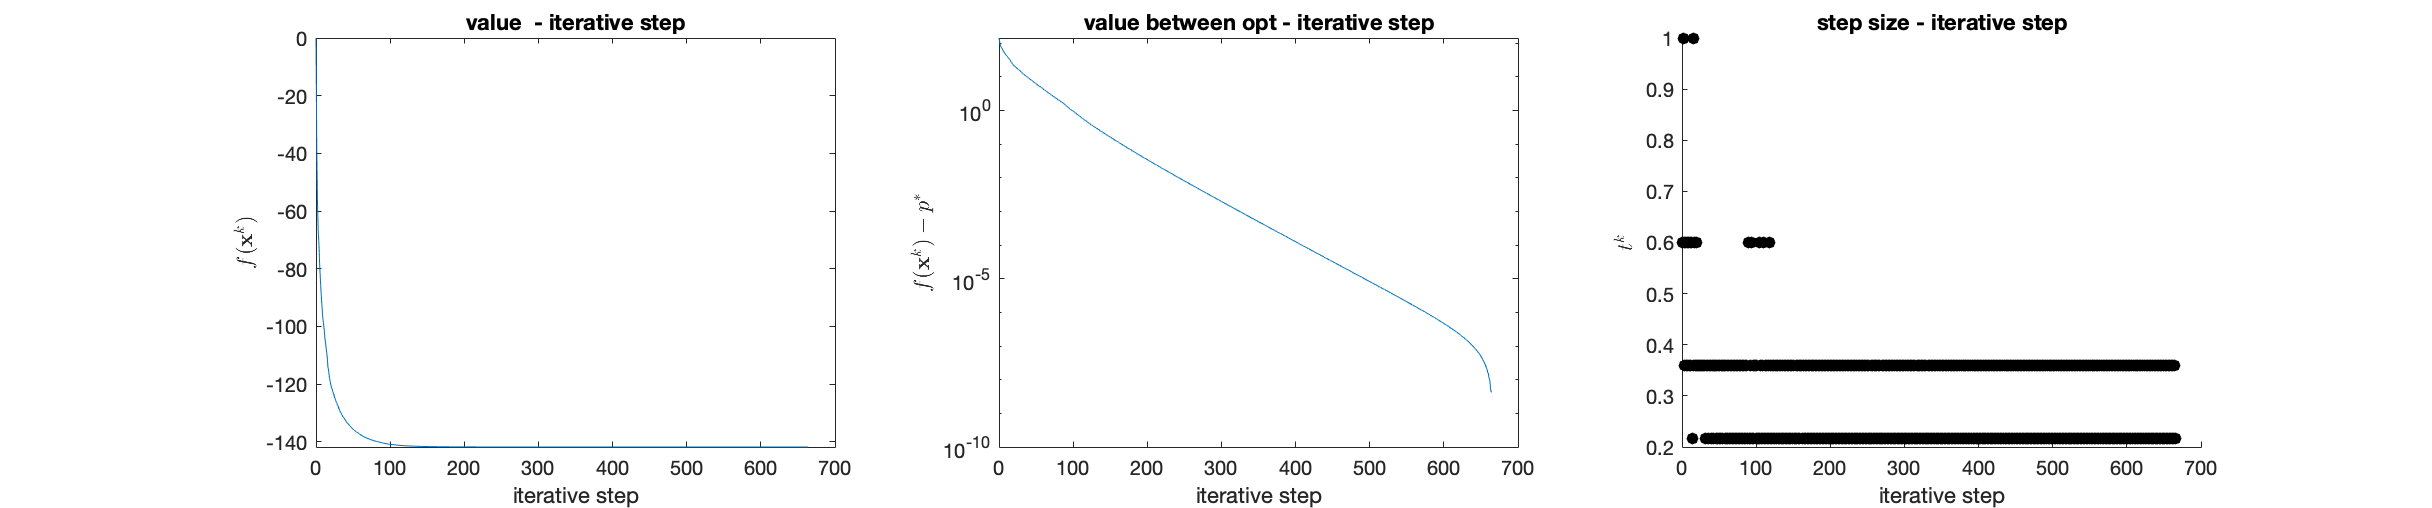
\includegraphics[width=350pt,keepaspectratio]{dntapp2_small_normal}
	\caption{Instance 1,small instance}
\end{figure}

\begin{figure}[H]
	\centering
	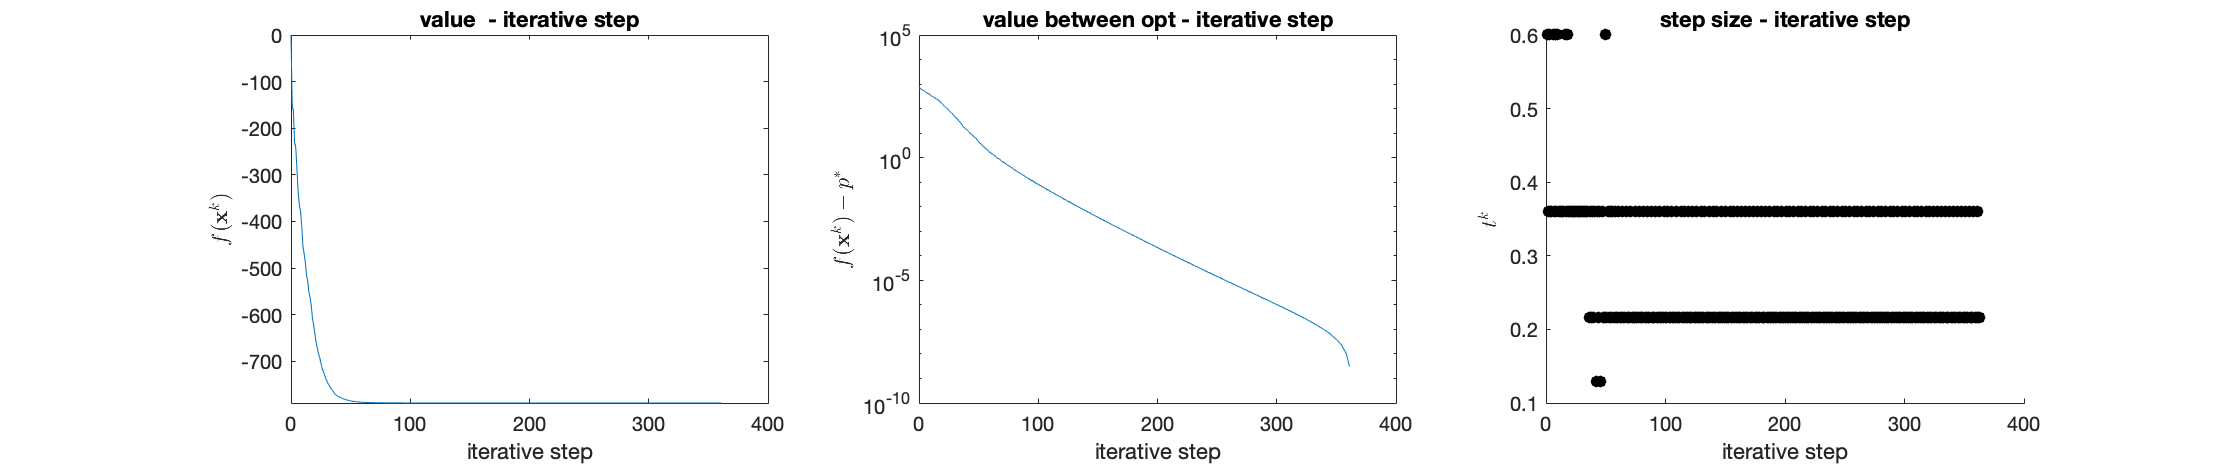
\includegraphics[width=350pt,keepaspectratio]{dntapp2_large_normal}
	\caption{Instance 2,large instance}
\end{figure}
 From the resule can we know that , the iterative step remains large compared with damped Newton Method.
\end{document}
